\section{Introduction}
\begin{frame}{Overview}
Goal: Fabricate shapes with desired deformation properties.

(i.e. The fabricated shape should match the target deformation under a particular
load.)

(Extra challenge: using only one material)
\end{frame}

\begin{frame}
\begin{figure}
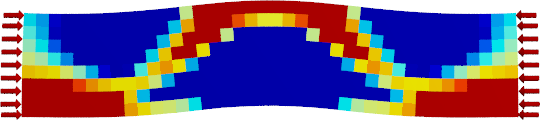
\includegraphics[width=0.7\textwidth]{Images/material_opt_bump_half.png}

\vspace{3mm}
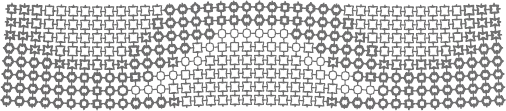
\includegraphics[width=0.7\textwidth]{Images/microstructure_bump_half_box.png}
\end{figure}

\begin{enumerate}
\item Find material properties that achieves the goal.
\item Find geometry that achieves these material properties.
\end{enumerate}
\end{frame}
